\chapter{Pewarisan Sifat}\label{ch:g9:heredity-and-traits}

Foto keluarga adalah data \omterm{def:g1:living-or-not:living}{biologi}. Dagu nenek pada anak
balitanya, rambut ikal ibunya yang tidak muncul pada satu
anak pun, satu kakak jangkung dan satu lagi tidak ---
keserupaan mengalir di dalam keluarga, dan begitu pula
perbedaannya. Buku ini sudah bersandar pada kenyataan itu
bertahun-tahun (anak kuda pada
\cref{rem:g4:animal-reproduction:mix}, adik-kakak pada
\cref{prop:g8:sexual-reproduction:shuffle}); bab pembuka
tahun ini akhirnya mempelajarinya: apa persisnya yang
diwariskan, apa yang tidak, dan apa yang dapat kita
simpulkan dari pola keserupaan keluarganya.

\begin{omfigure}
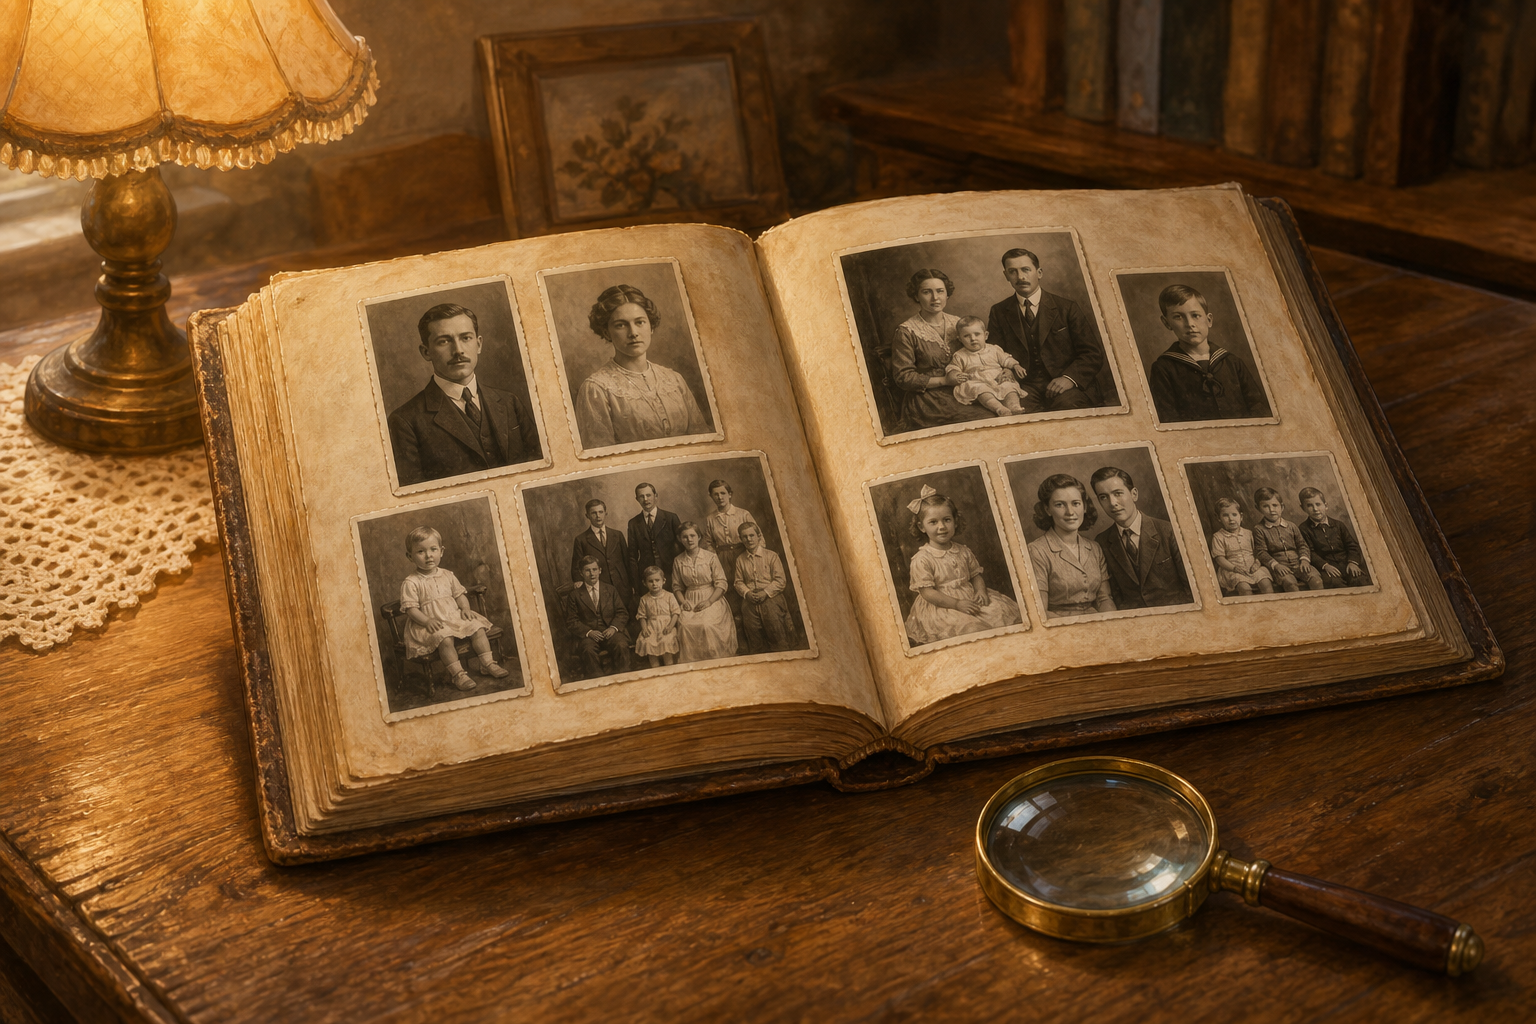
\includegraphics[width=0.62\linewidth]{images/book1/ai/g9-family-album.png}

{\small Data \omterm{def:g1:living-or-not:living}{biologi}, edisi sepia: keserupaan dan
perbedaan, yang mengalir menuruni angkatannya.}
\end{omfigure}

\section{Sifat, dan asalnya}

\begin{definition}[Sifat]\label{def:g9:heredity-and-traits:traits}
Sebuah \emph{sifat}\index{sifat} adalah ciri apa pun pada
seorang individu yang dapat diperikan: warna \omterm{def:g1:the-five-senses:sense}{mata}, golongan
\omterm{prop:g4:journey-of-food:absorb}{darah}, bentuk cuping \omterm{def:g1:the-five-senses:sense}{telinga}, tinggi badan, suara nyanyian,
sebuah parut. Seluruh kumpulan sifat individunya dibangun
oleh dua kerja: apa yang \emph{diwariskan}, dan apa yang
ditambahkan \emph{\omterm{def:g6:exploring-our-environment:components}{lingkungan} dan kehidupannya} (dunia pada
\cref{def:g4:adapted-to-their-world:adaptation}, yang
bekerja pada satu tubuh).
\end{definition}

\begin{definition}[Pewarisan sifat]\label{def:g9:heredity-and-traits:heredity}
Yang disebut \emph{pewarisan sifat}\index{pewarisan sifat}
adalah penerusan \omterm{def:g9:heredity-and-traits:traits}{sifat} dari induk kepada keturunannya lewat
reproduksi --- lewat, sebagaimana diperlihatkan
\cref{ch:g8:sexual-reproduction}, dua \omterm{def:g5:first-look-at-cells:cell}{sel} tunggal. \omterm{def:g9:heredity-and-traits:traits}{Sifat}
yang lewat dengan cara ini adalah \emph{sifat
turunan}\index{sifat turunan}: warna \omterm{def:g1:the-five-senses:sense}{mata} dan golongan \omterm{prop:g4:journey-of-food:absorb}{darah}
termasuk; parut dan \omterm{def:g1:the-five-senses:sense}{telinga} bertindik tidak, seberapa lama
pun dipakai. Uji pemilahannya adalah \omterm{def:g8:sexual-reproduction:gametes}{gametnya}: apa yang tak
dapat diangkut dua \omterm{def:g5:first-look-at-cells:cell}{sel}, tak dapat diteruskan keluarganya.
\end{definition}

\begin{example}[Memilah sebuah album keluarga]\label{ex:g9:heredity-and-traits:album}
Foto sang kakek: hidungnya yang khas --- turunan, itu dia
lagi pada bibi dan sepupunya; \omterm{def:g1:the-five-senses:sense}{kulitnya} yang cokelat terbakar
sebagai petani --- perolehan, cucunya yang bekerja di kantor
tidak punya; tingginya --- sebagian keduanya, sebab cucunya
melampauinya pada kerangka yang sama, disuapi tahun yang
lebih kaya (\cref{prop:g3:balanced-diet:jobs}); kepiawaian
biolanya --- bukan turunan sebagai keterampilan
(\cref{ex:g8:nervous-communication:juggler}: sinapsisnya
dilatih, bukan diteruskan), walaupun keluarga pemusiknya
memberi tahu kita bahwa sesuatu yang lebih halus sedang
bekerja pada apa yang diteruskan: mungkin bakatnya, tidak
pernah kabel terlatihnya sendiri.
\end{example}

\begin{proposition}[Turunan dan perolehan]\label{prop:g9:heredity-and-traits:sorting}
Kedua kerjanya terpisah pada tiga uji:
\begin{enumerate}
  \item \emph{pola keluarganya}: \omterm{def:g9:heredity-and-traits:heredity}{sifat turunan} berulang
        menembus pohonnya di sepanjang garis reproduksinya;
        \omterm{def:g9:heredity-and-traits:traits}{sifat} perolehan mengikuti kehidupannya (semua
        pelautnya terbakar matahari, siapa pun orang tuanya);
  \item \emph{hadir sejak awalnya}: golongan \omterm{prop:g4:journey-of-food:absorb}{darahnya}
        dipatok pada \omterm{def:g5:flower-to-fruit:steps}{pembuahan}; \omterm{def:g1:the-five-senses:sense}{kulit} terbakar dan
        keterampilannya dibangun sesudahnya;
  \item \emph{penerusannya}: anak orang yang diamputasi
        punya \omterm{def:g1:my-body:parts}{anggota geraknya}; anak binaragawan mulai tanpa
        latihan. \omterm{def:g9:heredity-and-traits:traits}{Sifat} perolehan mati bersama pemerolehnya
        --- \omterm{def:g8:sexual-reproduction:gametes}{gametnya} tidak mengangkutnya.
\end{enumerate}
Sebagian besar \omterm{def:g9:heredity-and-traits:traits}{sifat} yang terlihat --- tinggi badan,
perawakan, bahkan perangai --- ditenun dari kedua kerjanya,
rentang yang diwariskan dan pengisian yang dijalani.
\end{proposition}
\admitted

\section{Membaca pola keluarganya}

\begin{example}[Sifat yang melompat]\label{ex:g9:heredity-and-traits:skip}
Sebagian polanya membingungkan pada pandangan pertama: dua
orang tua bermata cokelat dengan seorang anak bermata biru;
\omterm{def:g9:heredity-and-traits:traits}{sifat} neneknya tidak ada pada satu anak pun namun kembali
pada seorang cucunya. Melompat itu lazim, dan ia membawa
sebuah kesimpulan yang berat: seorang tua dapat
\emph{meneruskan apa yang tidak diperlihatkannya}. Petunjuk
\omterm{def:g9:heredity-and-traits:traits}{sifat} itu berjalan tersembunyi menembus satu angkatan ---
sehingga yang diwariskan bukanlah \omterm{def:g9:heredity-and-traits:traits}{sifatnya} sendiri melainkan
sesuatu yang \emph{menentukannya}, terangkut tanpa terlihat.
\end{example}

\begin{proposition}[Apa yang dipaksakan polanya kepada kita]\label{prop:g9:heredity-and-traits:conclusions}
Tiga kesimpulan, masing-masing dipaksa sebuah pengamatan:
\begin{enumerate}
  \item karena \omterm{def:g9:heredity-and-traits:traits}{sifat} perolehan tidak lewat, yang lewat
        pastilah \emph{penentu} --- petunjuk untuk membangun
        \omterm{def:g9:heredity-and-traits:traits}{sifatnya}, bukan \omterm{def:g9:heredity-and-traits:traits}{sifatnya} sendiri;
  \item karena \omterm{def:g9:heredity-and-traits:traits}{sifatnya} melompati angkatan, penentunya dapat
        \emph{diangkut tanpa terlihat}: tiap individu
        mengangkut lebih banyak daripada yang ditampilkannya;
  \item karena setiap anak menerima dari kedua orang tuanya
        lewat dua \omterm{def:g8:sexual-reproduction:gametes}{gamet}
        (\cref{prop:g8:sexual-reproduction:core}), tiap
        orang tua menyumbangkan sebuah \emph{pilihan} dari
        penentunya --- dan pilihannya berbeda dari anak ke
        anak, kalau tidak adik-kakaknya akan serupa
        (pengocokan pada
        \cref{prop:g8:sexual-reproduction:shuffle}, kini
        ditemukan tempatnya: ia pengocokan \emph{atas
        penentunya}).
\end{enumerate}
\end{proposition}
\admitted

\begin{remark}[Pertanyaan yang ditimbulkannya]\label{rem:g9:heredity-and-traits:question}
Album keluarganya sudah menyudutkan kita pada sebuah
pertanyaan yang menakjubkan. Di suatu tempat di dalam
hampir-tidak-ada-apa-apanya \omterm{def:g8:reproductive-systems:male}{sel sperma}
(\cref{ex:g8:reproductive-systems:sperm} --- sebuah \omterm{def:g6:cell-unit-of-life:parts}{inti sel}
yang padat dan sebuah ekor) berjalan petunjuk untuk sebuah
hidung, sebuah golongan \omterm{prop:g4:journey-of-food:absorb}{darah}, sebuah warna \omterm{def:g1:the-five-senses:sense}{mata} --- dapat
diangkut tanpa diperlihatkan, dapat dipilih separuh-separuh,
dapat dibaca oleh tubuh yang sedang tumbuh. \emph{Di mana ia
berada, dan terbuat dari apa?} Anatomi spermanya sudah
menunjuk jawabannya: segala yang dikirim ayahnya muat di
dalam sebuah \omterm{def:g6:cell-unit-of-life:parts}{inti sel}
(\cref{rem:g5:first-look-at-cells:nucleus} menjanjikan bahwa
titik itu penting). Dua bab berikutnya membukanya.
\end{remark}

\begin{method}[Mengaudit sebuah sifat]\label{met:g9:heredity-and-traits:audit}
Untuk \omterm{def:g9:heredity-and-traits:traits}{sifat} apa pun, jalankan ketiga ujinya:
\begin{enumerate}
  \item petakan pada pohon keluarganya: apakah ia mengikuti
        garis reproduksinya, atau kehidupan dan kebiasaannya?
  \item tanggali: dipatok sejak awalnya, atau dibangun di
        sepanjang jalannya?
  \item terapkan uji \omterm{def:g8:sexual-reproduction:gametes}{gametnya}: dapatkah dua \omterm{def:g5:first-look-at-cells:cell}{sel}
        mengangkutnya? (sebuah parut tidak; golongan \omterm{prop:g4:journey-of-food:absorb}{darah} ya);
  \item vonisnya: turunan, perolehan, atau --- yang paling
        lazim --- sebuah rentang turunan, yang dijalani.
\end{enumerate}
\end{method}

\section{Latihan}

\begin{exercise}[$\star$]\label{exo:g9:heredity-and-traits:1}
Rumuskan \omterm{def:g9:heredity-and-traits:traits}{sifat} dan \omterm{def:g9:heredity-and-traits:heredity}{pewarisan sifat}, lalu berikan uji
pemilahannya dalam satu frasa.
\end{exercise}

\begin{exercise}[$\star$]\label{exo:g9:heredity-and-traits:2}
Golongkan: golongan \omterm{prop:g4:journey-of-food:absorb}{darah}; \omterm{def:g1:the-five-senses:sense}{telinga} bertindik; bintik-bintik;
bahasa Prancis yang lancar; bentuk cuping \omterm{def:g1:the-five-senses:sense}{telinga}.
\end{exercise}

\begin{exercise}[$\star$]\label{exo:g9:heredity-and-traits:3}
Nyatakan ketiga uji pada
\cref{prop:g9:heredity-and-traits:sorting}.
\end{exercise}

\begin{exercise}[$\star$]\label{exo:g9:heredity-and-traits:4}
Mengapa anak binaragawan mulai tanpa latihan? Apa yang
diperlihatkannya?
\end{exercise}

\begin{exercise}[$\star$]\label{exo:g9:heredity-and-traits:5}
Sebuah \omterm{def:g9:heredity-and-traits:traits}{sifat} yang melompat membuktikan seorang tua dapat apa?
\end{exercise}

\begin{exercise}[$\star$]\label{exo:g9:heredity-and-traits:6}
Mengapa yang diwariskan haruslah penentu alih-alih \omterm{def:g9:heredity-and-traits:traits}{sifatnya}?
Satu kalimat.
\end{exercise}

\begin{exercise}[$\star\star$]\label{exo:g9:heredity-and-traits:7}
Tinggi badan berjalan lebih tinggi pada cucunya di kerangka
yang sama. Uraikan kedua kerja pada kalimat itu.
\end{exercise}

\begin{exercise}[$\star\star$]\label{exo:g9:heredity-and-traits:8}
Jelaskan mengapa adik-kakak berbeda, dalam bahasa
penentunya --- dan mengapa kembar identik
(\cref{exo:g8:from-egg-to-birth:10}) tidak.
\end{exercise}

\begin{exercise}[$\star\star$]\label{exo:g9:heredity-and-traits:9}
Jalankan \cref{met:g9:heredity-and-traits:audit} pada: (a)
uban dini yang berulang pada sebuah keluarga; (b) daya tahan
seorang pemain sepak bola.
\end{exercise}

\begin{exercise}[$\star\star$]\label{exo:g9:heredity-and-traits:10}
Kasus biolanya: apa yang mungkin diteruskan keluarga
pemusiknya, kalau tidak pernah keterampilan terlatihnya?
Bedakan dengan cermat.
\end{exercise}

\begin{exercise}[$\star\star$]\label{exo:g9:heredity-and-traits:11}
Dua orang tua bermata cokelat, seorang anak bermata biru ---
dan tetangganya meragukan keluarganya. Belalah keluarganya
dengan logika \cref{ex:g9:heredity-and-traits:skip}.
\end{exercise}

\begin{exercise}[$\star\star\star$]\label{exo:g9:heredity-and-traits:12}
Dari anatomi \omterm{def:g8:reproductive-systems:male}{sel spermanya} saja
(\cref{ex:g8:reproductive-systems:sperm}), berhujahlah
tentang di mana penentu ayahnya pasti duduk --- dan ukuran
apa yang disiratkannya bagi petunjuk seorang manusia utuh.
\end{exercise}

\section{Soal: Sang Ahli Silsilah Desa}

\begin{problem}[{Soal akhir pekan --- tiga angkatan, satu
buku besar sifat}]\label{pb:g9:heredity-and-traits:1}
Seorang ahli silsilah desa memberi catatan pada pohon
keluarga parokinya dengan \omterm{def:g9:heredity-and-traits:traits}{sifat}: ``dagu kapel'' (sebuah dagu
khas yang berulang selama seabad), kidal, batuk paru
berdebu tepung para pembuat rotinya, golongan \omterm{prop:g4:journey-of-food:absorb}{darah} dari
daftar donornya, dan wajah terbakar matahari para gembalanya.

\medskip\noindent\textbf{Bagian I --- Memilah buku
besarnya.}
\begin{enumerate}
  \item Pilahlah kelima \omterm{def:g9:heredity-and-traits:traits}{sifatnya} dengan
        \cref{met:g9:heredity-and-traits:audit}, beserta uji
        yang menentukan bagi masing-masing.
  \item Batuknya mengikuti toko rotinya, bukan keluarganya:
        menikah masuk membawanya, pindah pergi
        kehilangannya. Uji yang mana ini, sedang bekerja?
  \item Dagu kapelnya melompati angkatan tengah pada dua
        cabang. Tariklah kesimpulan yang dipaksakannya.
  \item Golongan \omterm{prop:g4:journey-of-food:absorb}{darahnya} kadang mengejutkan daftarnya:
        seorang anak bergolongan O dari orang tua bergolongan
        A dan B. Apa yang pasti diangkut tiap orang tuanya?
\end{enumerate}

\medskip\noindent\textbf{Bagian II --- Bacaan
penentunya.}
\begin{enumerate}[resume]
  \item Tulis ulang seabad dagunya dalam bahasa penentu: apa
        yang sebenarnya berjalan menuruni empat angkatan, di
        dalam kendaraan yang mana
        (\cref{def:g9:heredity-and-traits:heredity})?
  \item Mengapa para sepupu pembawa dagunya berbeda dalam
        segala hal lainnya? Temukan pengocokannya.
  \item Sang ahli silsilah tidak menemukan satu kasus pun
        --- dalam seabad --- tentang sebuah parut, sebuah
        pekerjaan atau sebuah bahasa yang lewat kepada
        seorang bayi. Nyatakan penyamarataannya, dan
        alasannya setingkat mekanisme.
  \item Kembar satu keluarga serupa sampai ke dagunya dan
        lebih jauh lagi. Apa yang disimpulkan buku besarnya
        tentang permulaannya
        (\cref{rem:g5:human-reproduction:twins})?
\end{enumerate}

\medskip\noindent\textbf{Bagian III --- Ceramahnya.}
\begin{enumerate}[resume]
  \item Sang ahli silsilah berceramah: ``parokinya
        meneruskan dua warisan --- satu lewat \omterm{def:g8:sexual-reproduction:gametes}{gamet}, satu
        lewat hidup bersama.'' Tetapkan kelima \omterm{def:g9:heredity-and-traits:traits}{sifat} buku
        besarnya pada kedua salurannya.
  \item ``Kita masing-masing menampilkan lebih sedikit
        daripada yang kita angkut.'' Belalah dari buku
        besarnya, dua kali.
  \item Seorang pendengar bertanya, secara ragawi petunjuk
        pada saluran \omterm{def:g8:sexual-reproduction:gametes}{gametnya} itu apa. Berikan jawaban jujur
        pada \cref{rem:g9:heredity-and-traits:question}
        --- letaknya diketahui, isinya bab berikutnya.
  \item Tutuplah ceramahnya dengan vonis satu baris auditnya
        atas kasus yang paling lazim: sebagian besar \omterm{def:g9:heredity-and-traits:traits}{sifat}
        adalah \emph{apa}, yang dijalani \emph{bagaimana}?
\end{enumerate}
\end{problem}
